%! TeX program = lualatex
\documentclass[../main.tex]{subfiles}
\begin{document} \section{Review of inverse functions}
  Intuitively, the inverse of a function \(f(x)\) is another function \(g(x)\) that undoes whatever \(f(x)\) does to its input. This intuition is not precise enough to be useful. Let's start with the definition.

  \begin{mdframed}[style=withref-compact]
    Given a function \(f\) whose domain is \(D\) and range is \(R\), its \hlmain{inverse function} (if it exists) is \hlsupp{the} function \(f^{-1}(x)\) such that
    \[
      f^{-1}(f(x)) = x \text{ on } D \quad\text{and}\quad f(f^{-1}(x)) = x \text{ on } R.
    \]

    \textbook{Page 78}
  \end{mdframed}

  {\faExclamationTriangle{} \(f^{-1}(x)\) is NOT \(\tfrac{1}{f(x)}\). To write \(\tfrac{1}{f(x)}\) as a power, write \(\tfrac{1}{f(x)} = f(x)^{-1}\) or \(\tfrac{1}{f(x)} = \big( f(x) \big)^{-1}\).}
  \bigskip

  This definition is \hlinfo{actually very useful}. This definition \emph{alone} tells us how to
  \begin{enumerate}[noitemsep]
    \item check whether two functions are inverses of each other, 
    \item determine whether a function has an inverse graphically, 
    \item sketch the inverse function, 
    \item find inverses (graphically and algebraically) if possible,
    \item find inverses (graphically and algebraically) by restricting the domain, and
    \item avoid subtle mistakes.
  \end{enumerate}

  We skip the trial-and-error part of the story and go straight to the \hlinfo{insight}: Let's pretend \(f(x)\) has an inverse and denote \underline{\hspace{2in}}. The definition now gives us an useful equation:
  \blanklines{19}

  To evaluate \(y = f^{-1}(x)\) is to \underline{\hspace{4in}}. For example, \(\log_{2}(x)\) is the inverse of \(2^{x}\) and to evaluate \(\log_{2}(8)\) means to 
  \blanklines{4}

  \begin{example}
    Are \(f(x) = (x+1)^{3} - 2\) and \(g(x) = (x+2)^{1/3} - 1\) inverses of each other?
    \blanklines{5}
  \end{example}

  \begin{example}
    Sketch the inverse of given functions if it exists.

    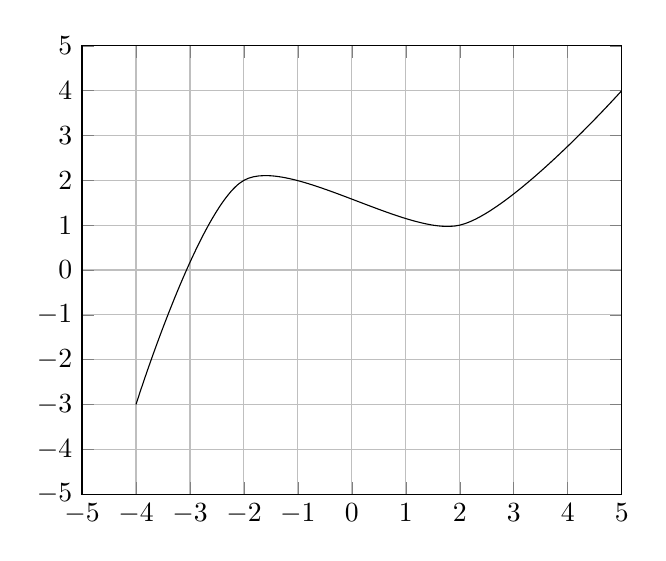
\begin{tikzpicture}
      \begin{axis}[xmin=-5, xmax=5, ymin=-5, ymax=5, xtick={-5,-4,...,5}, ytick={-5,-4,...,5}, grid=major]
        \addplot[smooth] coordinates {(-4,-3) (-2,2) (2,1) (5,4)};
      \end{axis}
    \end{tikzpicture}
    \includegraphics{../standalones/build/plot_empty_5x5}
    \medskip

    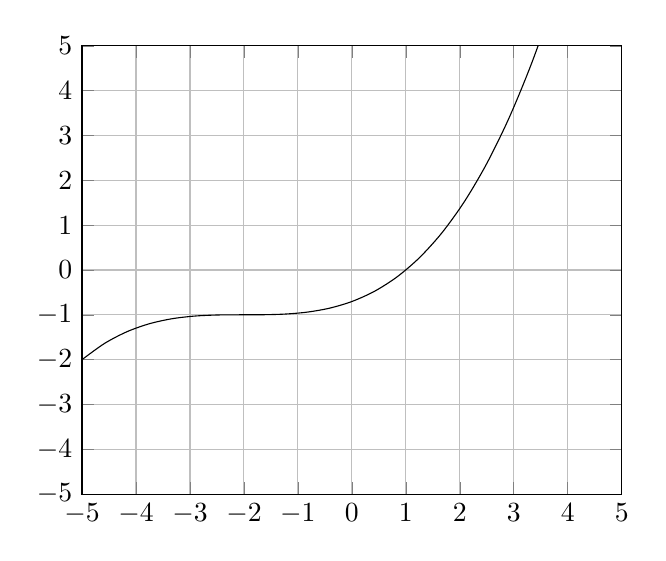
\begin{tikzpicture}
      \begin{axis}[xmin=-5, xmax=5, ymin=-5, ymax=5, xtick={-5,-4,...,5}, ytick={-5,-4,...,5}, grid=major]
        \addplot[smooth, domain=-5:5] {((x+2)/3)^3 - 1};
      \end{axis}
    \end{tikzpicture}
    \includegraphics{../standalones/build/plot_empty_5x5}
  \end{example}

  \begin{example}
    Are \(x^{2}\) and \(\sqrt{x}\) inverses of each other? Assume \(x^{2}\) is defined for all real numbers.
    \blanklines{10}
  \end{example}
  \clearpage

  \begin{example}
    Find the inverse of \(\frac{(x - 3)^{4}}{2}\), restrict the domain if necessary.  Determine the domain and range of its inverse. 

    \blanklines{10}
  \end{example}

  \begin{example}
    Sketch \(\cos(x)\) on \([-2\pi, 2\pi]\). Clearly label the axes.

    Define \(\arccos(x)\) by sketching its graph. What is the domain and range of \emph{your} \(\arccos(x)\)?

    \begin{minipage}{3in}
      \begin{tikzpicture}
        \begin{axis}[
          ymin={-3}, ymax={3},
          xmin={-2*pi}, xmax={2*pi},
          ytick={4},
          xtick={-2*pi, 2*pi},
          xticklabels={\(-2\pi\), \(2\pi\)}, yticklabels={},
          ]

          % \addplot[main, thick, smooth, samples=1000, domain={-2*pi-pi/6}:{2*pi+pi/6}] {sin(x)};
        \end{axis}
      \end{tikzpicture}
    \end{minipage}
    \begin{minipage}{4in}
      \blanklines{9}
    \end{minipage}
  \end{example}

  The inverses of \(\sin(x), \cos(x), \tan(x)\) and so on are called \emph{inverse trigonometric function}. Because all basic trig functions fails the horizontal line test, we need to restrict the domain.
  \medskip
  \begin{align*}
    y &= \sin^{-1}(x) \text{ is defined for } \underline{\hspace{2in}} \\[3ex]
    y &= \cos^{-1}(x) \text{ is defined for } \underline{\hspace{2in}} \\[3ex]
    y &= \tan^{-1}(x) \text{ is defined for } \underline{\hspace{2in}}
  \end{align*}
  Make sure to review all other inverse trigonometric functions on your own.
  \bigskip

  To evaluate an inverse trig function is to solve the original trig function \hlmain{with restriction}!

  \begin{example}
    Evaluate \(\cos^{-1}(\cos(2\pi))\). 
    \blanklines{10}
  \end{example}

  \begin{example}
    Evaluate \(\tan^{-1}\left(\frac{\sqrt{3}}{3}\right)\).
    \blanklines{10}
  \end{example}

\end{document}

